\chapter{Atomes de Rydberg alcalins en interaction}
\label{chapter:Rydberg}
%Atomes de Rydberg : à bas $l$ ou circulaires

Un atome de Rydberg est un atome dont un électron au moins occupe un état de grand nombre quantique principal $n$.
Par là, un atome de Rydberg présente des propriétés physiques surdimensionnées par rapport à un atome non excité ou peu excité.
On le remarque tout d'abord sur sa taille : un atome de rubidium dans le niveau $n=110$ a une extension spatiale de l'ordre d'$1 ~\si{\micro\meter}$, vingt mille fois plus grand que le rayon de Bohr qui représente l'ordre de grandeur caractéristique de la taille d'un atome dans son état fondamental.

Avec un électron à une telle distance du c\oe ur atomique, les atomes de Rydberg présentent de très grands moments dipolaires de transition entre états de Rydberg voisins. On comprend dès lors leur très grande sensibilité au rayonnement électromagnétique \cite{ENS_ENHANCED}.
Ces très grands moments dipolaires de transition engendrent également de très forts couplages entre atomes de Rydberg voisins par l'intermédiaire de l'interaction dipolaire. Ces couplages sont eux aussi plusieurs ordres de grandeur plus importants que ceux qui se manifestent entre des atomes dans le niveau fondamental.
L'interaction dipolaire entre atomes de Rydberg est au c\oe ur des travaux de recherche présentés dans cette thèse. C²e premier chapitre vise à en apporter les éléments théoriques importants pour la compréhension des résultats et discussions qui seront abordés par la suite.

La première partie de ce chapitre décrit la théorie du défaut quantique \cite{TXT_GALLAGHER}, qui permet de calculer les énergies propres des états de Rydberg et leur fonction d'onde radiale loin du c\oe ur atomique positif.
Il est alors aisé de calculer les éléments de matrice de l'opérateur de dipôle électrique entre deux niveaux de Rydberg.
Connaître les dipôles de transition entre un niveau de Rydberg et les niveaux voisins est essentiel au calcul des interactions dipolaires entre deux atomes de Rydberg, ce que nous aborderons dans un deuxième paragraphe.
Enfin, nous verrons le détail de cette interaction dans deux cas particuliers  : les atomes de Rydberg en interaction autour du niveau $60$S et les atomes de Rydberg en interaction autour du niveau circulaire $50$C.
Ces deux cas particuliers seront à nouveau discutés plus en détail dans des chapitres dédiés aux expériences que nous avons menées.

\section{Les atomes de Rydberg alcalins : des hydrogénoïdes géants}
Un atome de Rydberg alcalin a un seul électron dans un niveau de grand nombre quantique principal $n$. L'essentiel de la fonction d'onde de cet électron est localisé dans des régions atomiques éloignées du c\oe ur, c'est-à-dire de l'ensemble du noyau atomique et des couches électroniques inférieures.
Pour cette raison, il ressemble à un atome d'hydrogène, dont l'unique électron voit un c\oe ur protonique simple de charge totale $+q=\numv{1.602176565(35)d-19}\si{\coulomb}$ \cite{MX_CODATA14}.
Dans le cas de l'hydrogène, ce c\oe ur est plusieurs ordres de grandeurs plus petit que la taille typique de l'orbite de l'électron : le niveau électronique fondamental $1$S a un \og rayon \fg{} caractéristique $a_0 = \numv{0,52917721092(17)}\si{\angstrom}$ \cite{MX_CODATA14}, alors que le proton a un rayon $r_p = \numv{0.8775(51)}\si{\femto\meter}$ \cite{MX_CODATA14}.

Les cinq ordres de grandeur séparant le rayon de l'orbite électronique et le rayon du proton permettent de considérer que le potentiel vu par l'électron est parfaitement coulombien sur tout l'espace.
Les énergies propres de l'atome d'hydrogène sont alors données par
\begin{equation}\label{eq:Hatom}
E(n,l,j)= - \frac{E_I}{n^2} ,
\end{equation}

avec
\begin{equation}\label{eq:E_I}
E_I = \frac{1}{1+\frac{m_e}{M}}\frac{m_e q^4}{32\pi^2 \epsilon _0^2 \hbar ^2}
\end{equation}
l'énergie d'ionisation pour l'électron dans le niveau $1$S de l'atome d'hydrogène, où $M$ est la masse du c\oe ur atomique (masse d'un proton pour l'atome d'hydrogène, masse atomique $m_{Rb87}$ pour l'atome de $^{87}Rb$ dans un état de Rydberg), $n$ le nombre quantique principal, $m_e$ la masse de l'électron, $\epsilon_0$ la permittivité diélectrique du vide, et $\hbar$ la constante de Planck réduite.

Les états propres de ce modèle s'écrivent en coordonnées sphériques comme le produit d'une partie radiale, fonction de $r$ qui est la distance de l'électron au c\oe ur atomique, par une partie angulaire, fonction des coordonnées angulaires $\theta$ et $\phi$ \cite{TXT_COHEN1FR} : 
\begin{equation}\label{eq:Hfonctonde}
\psi(r,\theta,\phi) = R_{nl}(r)\cdot Y_l^{m_l}(\theta,\phi).
\end{equation}
Ici, $l$ est le nombre quantique orbital et $m_l$ le nombre quantique magnétique, associé à la projection du moment angulaire orbital de l'électron sur l'axe de quantification.
Cette première description ne prend pas en compte les corrections aux énergies dues au couplage entre le moment magnétique intrinsèque de l'électron, son spin, et son moment magnétique orbital, ce que l'on dénomme couplage fin.
Elle néglige tout autant le couplage entre le moment magnétique total de l'électron et le moment magnétique du c\oe ur atomique, le couplage hyperfin \cite{TXT_COHEN2FR}.

En présence de couplage fin, les bons nombres quantiques deviennent $n,l,j,m_j$, avec $j=l+s$ où $s=1/2$ est le moment magnétique de spin de l'électron. Le couplage hyperfin étant très petit pour les niveaux de Rydberg, nous en ferons fi et continuerons d'utiliser la base avec moment cinétique total de l'électron $j$ pour décrire les niveaux électroniques.

En comparaison avec l'atome d'hydrogène, le c\oe ur positif de l'atome de Rydberg alcalin comporte une structure d'extension spatiale bien plus importante \cite{TXT_GALLAGHER}.
Dans la région des couches électroniques inférieures, le potentiel est bien plus profond que le potentiel coulombien car l'effet d'écrantage partiel de la charge totale positive du c\oe ur par les électrons internes disparaît lorsque l'on s'en approche : c'est l'effet de pénétration du c\oe ur.
Ensuite, la distribution spatiale des charges positives et négatives entraîne une polarisabilité du c\oe ur composé.
L'électron de Rydberg interagit avec cette distribution de charge complexe, ce qui modifie sa fonction d'onde et son énergie propre.
Afin de rendre compte de ces effets, il est nécessaire d'apporter une correction aux énergies propres de l'électron de Rydberg d'un atome alcalin : le défaut quantique.

	\subsection{Hamiltonien de l'atome de Rydberg et défaut quantique}
Les deux effets précédemment cités de pénétration du c\oe ur et de polarisabilité du c\oe ur peuvent être efficacement décrits par la théorie du défaut quantique. Celui-ci apparaît comme une correction $\delta_{nlj}$ au nombre quantique principal $n$ dans l'équation des énergies propres des niveaux électroniques \cite{TXT_GALLAGHER}, qui devient
\begin{equation}\label{eq:E_I_delta}
E(n,l,j) = \frac{- E_I}{(n-\delta_{nlj})^2} ,
\end{equation}
avec 
\begin{equation}\label{eq:deltanlj}
\delta(n,l,j)=\delta_{lj,0} + \frac{\delta_{lj,2}}{(n-\delta_{lj0})^2} + \frac{\delta_{lj,4}}{(n-\delta_{lj0})^4} + \frac{\delta_{lj,6}}{(n-\delta_{lj0})^6} + \cdots .
\end{equation}

\begin{table}[tph!]
	\centering
	\caption[Table des défauts quantiques du $^{87}Rb$ et $^{85}Rb$]{Défauts quantiques  du \Rb{85} extraits de \cite{MX_GALLAGHERSPECRBNSND03, MX_GALLAGHERSPECRBNF06} et du \Rb{87} extraits de \cite{MX_MACKNSNDRYD}}
	\label{tab:q_defect}
	\begin{tabular}{ c S[table-format=1.12]S[table-format=2.8]  S[table-format=1.10]S[table-format=2.6]}
		\toprule\midrule
		 &  \multicolumn{2}{c}{\Rb{85}}	&   \multicolumn{2}{c}{\Rb{87}}  \\ 
		 \midrule
				  &		$\delta_{lj,0}$				&	$\delta_{lj,2}$		&	$\delta_{lj,0}$			&	$\delta_{lj,2}$ \\ 
		\midrule
		$nS_{1/2}$&  	3.1311804(10)		&	0.1784(6) 	& 3.1311807(8)	& 0.1787(2)	\\
		$nP_{1/2}$&  	2.6548849(10)		&	0.2900(6)	&						&				\\
		$nP_{3/2}$&  	2.6416737(10)		&	0.2950(7)	&						&				\\
		$nD_{3/2}$&  	1.34809171(40)	&	-0.60286(26)&1.3480918(11)	&	-0.6054(4)	\\
		$nD_{5/2}$&  	1.34646572(30)	&	-0.59600(18)&1.3464622(11)	&-0.5940(4)		\\
		$nF_{5/2}$&  	0.0165192(9)		&	-0.085(9)	&						&				\\
		$nF_{7/2}$&  	0.0165437(7)		&	-0.086(7)	&						&				\\
%		$nG$	&0.00400(9)	&&&\\
%		$n,l>4$ & {$0.004(4/l)^5$}&&&\\
		\midrule
		\bottomrule
 	\end{tabular}
\end{table}
%
La série \eqref{eq:deltanlj} développe le défaut quantique en puissances de $1/(n-\delta_{lj,0}) = 1/n^*$ : $n^*$ est le nombre quantique principal corrigé du défaut quantique.
Ses coefficients, présentés en table \eqref{tab:q_defect}, sont extraits des mesures précises des fréquences de transition entre niveaux de Rydberg voisins \cite{ENS_SPECNA2,ENS_SPECCS,MX_MECHEDERYDSPECTRO87} et la série sous cette forme converge rapidement \cite{MX_MARTINSERIESSPECNA} :
pour les niveaux de $n>40$, les deux premiers termes suffisent à obtenir une précision meilleure que le $\si{\kilo\hertz}$ sur une large gamme de valeurs de $n$.
Les coefficients de la série sont fonction de $l$ et $j$, ainsi que de l'espèce atomique.
Nous n'avons pas connaissance de défauts quantiques mesurés pour le \Rb{87} autres que ceux présentés ici, mais l'utilisation de ceux du \Rb{85} fournit de bons résultats grâce à la grande similarité des structures électroniques de ces deux isotopes.
En ce qui concerne les niveaux de $l>3$, leurs défauts quantiques sont petits, et donc d'autant plus difficiles à mesurer. Ils seront donc négligés par la suite.
Avec les valeurs connues des défauts quantiques, nous obtenons des fréquences de transition entre niveaux de Rydberg voisins avec une précision meilleure que $\sim 50\si{\kilo\hertz}$.

Dans le cas extrême des niveaux de Rydberg circulaires, qui ont un moment orbital maximal $l=n-1$, le défaut quantique peut être considéré nul et alors on retrouve le modèle de l'atome d'hydrogène sans correction autre que la masse du c\oe ur.
		
	\subsection{Partie radiale de la fonction d'onde et calcul du dipôle de transition}
	Ayant ces outils à notre disposition, nous pouvons désormais nous employer à calculer les éléments de matrice de l'opérateur de transition dipolaire $\vec{d}=q\vec{r}$ entre niveaux de Rydberg, qui apparaît de façon essentielle dans les termes de couplage des atomes avec le rayonnement électromagnétique et dans le couplage dipolaire entre deux niveaux de Rydberg $\ket{n,l,j,m_j}$ et $\ket{n',l',j',m_j'}$. Ces éléments de matrice s'écrivent

	\begin{equation}\label{eq:matrixelements}
	\begin{aligned}
	\bra{nl,l,j,m_j}q\vec{r}\ket{n',l',j',m_j'}= & ~q\bra{n,l,j,m_j} r\frac{\vec{r}}{r} \ket{n',l',j',m_j'} \\
	= & ~q\cdot \int r^2dr~R^*_{nl}(r)~r~R_{n',l'}(r)~ \bra{l,j,m_j}\frac{\vec{r}}{r}\ket{l',j',m_j'} \\
	= & ~q.\mathcal{R}(nl,n'l').\mathcal{A}(ljm_j,l'j'm_j')	 ,
	\end{aligned}
	\end{equation}
	
\noindent c'est-à-dire comme produit d'une partie radiale $\mathcal{R}$ et d'une partie angulaire $\mathcal{A}$.
Or la partie radiale $R_{n,l}(r)$ de la fonction d'onde est affectée par l'effet de pénétration du c\oe ur décrit plus haut et doit donc être corrigée \cite{TXT_GALLAGHER}.
Le calcul de $\mathcal{R}$ peut être fait numériquement par une méthode dite de Numerov \cite[pp.10-24]{TXT_GALLAGHER}.
Cette méthode s'appuie sur le fait que le potentiel à l'extérieur du c\oe ur atomique reste coulombien. La partie radiale de la fonction d'onde peut donc y être calculée à partir de la même équation, avec les mêmes conditions aux limites à $r \rightarrow \infty$, mais avec une énergie totale différente qui est imposée par les défauts quantiques.

\begin{figure}[!h]
	\centering
	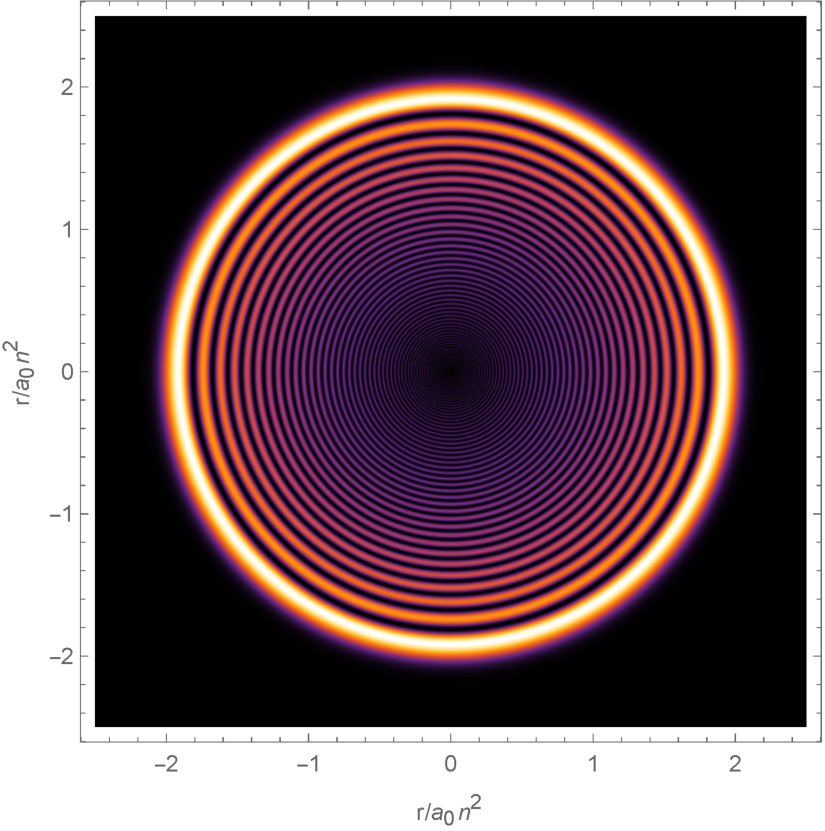
\includegraphics[width=0.6\linewidth]{figures/WaveFunc_60S_}
	\caption[Fonction d'onde du niveau 60S]{Probabilité de présence de l'électron dans le niveau $60$S.}
	\label{fig:wavefunc60S}
\end{figure}

La figure \eqref{fig:wavefunc60S} montre la probabilité de présence $r^2|R_{60\mathrm{S}}(r)|^2$ de l'électron de Rydberg dans le niveau $60$S du \Rb{87}.
Cela montre que la fonction d'onde se situe essentiellement loin du c\oe ur atomique et justifie donc la validité de la méthode de Numerov.

\`A partir du calcul de $R_{nl}(r)$, l'on peut aisément dériver la partie radiale de l'opérateur dipôle $\vec{d}$.
L'on apprend en particulier que la partie radiale de $\vec{d}$ entre deux niveaux de nombre quantique principal similaire varie comme $\mathcal{R} \sim a_0\cdot n^{*2}$.
Mentionnons ici que le rayon moyen de l'orbitale électronique d'un niveau de Rydberg est très similaire au calcul de la partie radiale de l'opérateur dipôle :
\begin{equation}\label{eq:orbital_size}
\braket{r_{\ket{n,l,j,m_j}}} = \int r^2dr~R_{nl}(r).r.R_{nl}(r) = \mathcal{R}(nl,nl)
\end{equation}
%\`A titre d'exemple, le niveau $60$S a ainsi un rayon moyen de $\braket{r} = 4850~a_0 = \numv{256.5}~\si{\nano\meter}$.

	\subsection{Temps de vie des niveaux de Rydberg}
Avec la connaissance des dipôles de transition d'un niveau de Rydberg vers les niveaux voisins, 	il est possible de connaître le temps de vie de celui-ci.
Deux processus entrent en jeu dans la désexcitation radiative à température finie de ces niveaux atomiques :
les transitions par émission spontanée mais aussi les transitions par absorption ou émission stimulée par le rayonnement de corps noir de leur environnement.
En effet, les transitions entre niveaux de Rydberg proches en énergie sont dans le domaine des micro-ondes millimétriques.
Cela implique qu'elles seront à considérer dès les très basses températures : contrairement aux photons optiques, des photons micro-ondes sont déjà émis par le rayonnement du corps noir aux températures cryogéniques, de quelques \si{\milli\kelvin} à quelques \si{\kelvin}.

\`A titre d'exemple, la fréquence de la transition entre le niveau $\ket{60\mathrm{S}1/2}$ et le niveau $\ket{59\mathrm{P}3/2}$ vaut $\nu = E/h = \numv{18.5213}\si{\giga\hertz}$. La température de corps noir correspondant à cette fréquence est de $T=h\nu /\kb = \numv{0.89}\si{\kelvin}$.
Cette transition sera donc limitante pour le temps de vie du niveau 60S dès lors que celui-ci sera dans un environnement dépassant les $\numv{500}\si{\milli\kelvin}$.

%Or les températures de rayonnement du corps noir associées à ces gammes de fréquence se situent dans la gamme de quelques \si{\milli\kelvin} à quelques \si{\kelvin}.
\`A température nulle, le temps de vie d'un niveau excité est calculé uniquement à partir des coefficients d'Einstein pour l'émission spontanée \cite{MX_GALLAGHERBBODY}. Un électron dans un niveau excité est couplé aux niveaux de plus basse énergie par les modes électromagnétiques du vide et le taux de désexcitation d'un niveau initial $\ket{i}$ vers un niveau final $\ket{f}$ séparés d'une énergie $E_f - E_i = -\hbar \omega_{if} < 0$ est donné par :
\begin{equation}\label{eq:EinsteinAif}
A_{if} = \frac{2\omega_{if}^3}{3\epsilon_0c^3h}\cdot q^2\cdot |\bra{i}r\ket{f}|^2
\end{equation}
Ce coefficient est le produit de la densité de modes du rayonnement électromagnétique autour de la fréquence résonante $\nu_{if}=\omega_{if}/2\pi$ et du moment dipolaire de transition entre les niveaux $\ket{i}$ et $\ket{f}$ couplés par ce rayonnement.
Le temps de vie de l'état excité est alors calculé en sommant les taux d'émission spontanée vers chacun des niveaux auxquels il a accès par transition dipolaire électrique.
Les transitions dipolaires par émission d'un photon respectant la règle de sélection $\Delta l = \pm1$ et $\Delta m \leq 1$, la quantité de termes à considérer s'en trouve heureusement limitée.

\`A température finie cependant, l'absorption et l'émission stimulée vers les niveaux voisins entrent en jeu.
Le coefficient d'Einstein pour l'absorption et  l'émission stimulée s'écrit ici
\begin{equation}\label{eq:EinsteinBif}
B_{if} = A_{if} \bar{n}(\omega_{if})
\end{equation}
Il s'agit alors de connaître, pour une température donnée, le taux d'occupation du rayonnement électromagnétique aux fréquences des transitions entre niveaux de Rydberg.
Ce taux nous est donné par la distribution de Bose-Einstein pour un gaz de bosons \cite{TXT_GORECKIPHYSTAT} :
\begin{equation}\label{eq:BoseStat}
\bar{n}(\omega) = \frac{1}{e^{\frac{\hbar\omega}{\kb T}}-1}
\end{equation}
qui devient, lorsque $\kb T \gg \hbar\omega$,
\begin{equation}\label{eq:BoseStat_blackbody}
\bar{n}(\omega) \sim \frac{\kb T}{\hbar\omega}.
\end{equation}
Le nombre de photons par mode varie alors linéairement avec la température et ces photons stimulent des transitions vers des niveaux de Rydberg proches, diminuant ainsi le temps de vie du niveau de départ.


	\subsection{Le niveau de Rydberg 60S : $\mathbf{\ket{n=60,l=0}}$}
Afin d'illustrer les propriétés singulières des niveaux de Rydberg, prenons un exemple qui nous sera utile par la suite : le niveau de Rydberg 60S, qui a donc un moment cinétique orbital $l=0$. Nous nous intéresserons à sa taille, à ses dipôles de transition avec les niveaux voisins, et à son temps de vie.

Grâce à l'équation \eqref{eq:orbital_size}, nous pouvons obtenir la taille de l'orbitale électronique dans le niveau 60S : son rayon moyen vaut $\braket{r} = 4850~a_0 = \numv{256.5}\si{\nano\meter}$.
%, valeur qui paraît très grande en comparaison avec l'extension spatiale d'un atome dans le niveau fondamental qui est de l'ordre de quelques $a_0$.

De par la règle de sélection $\Delta l=\pm1$, les termes à considérer pour les transitions dipolaires depuis le niveaux $\ket{n=60,l=0}$ sont les couplages avec les niveaux $n\mathrm{P}_j = \ket{n,l=1,j},~j\in\{1/2,3/2\}$.
La figure \eqref{fig:matrixelements} montre, pour tous les $n$, la somme des coefficients d'Einstein d'émission spontanée et d'absorption et émission stimulée à différentes températures vers les niveaux $n\mathrm{P}_j$.

\begin{figure}[th!]
	\centering
	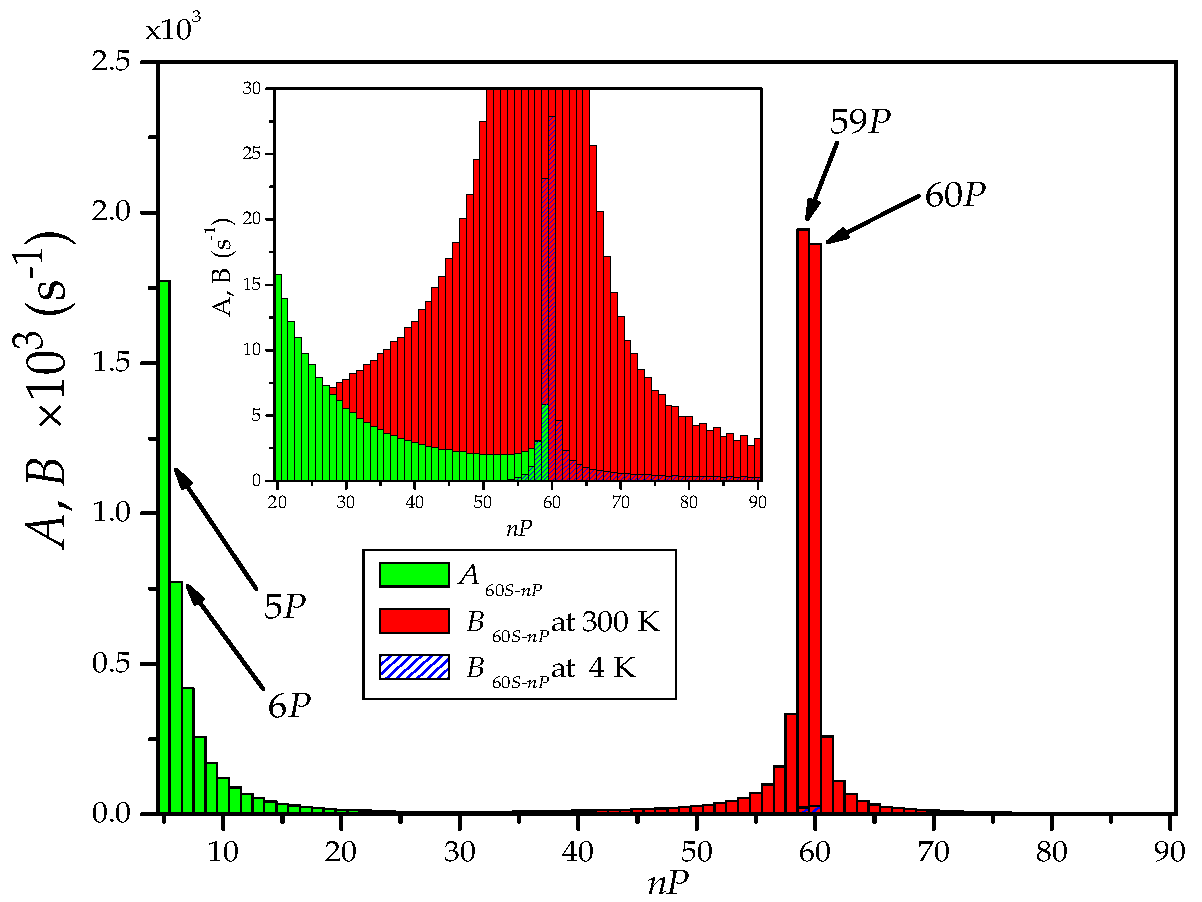
\includegraphics[width=0.7\linewidth]{figures/lifetime}
	\caption[Coefficients d'Einstein de 60S vers $n\mathrm{P}_j,j\in{1/2,3/2}$]{
	Coefficients d'Einstein pour l'émission spontanée (A) et pour l'absorption et émission stimulée par le rayonnement du corps noir(B), depuis le niveau 60S vers les niveaux $n\mathrm{P}_j$.
	Pour chaque $n$, nous montrons la somme des coefficients vers $n\mathrm{P}_{j=1/2}$ et $n\mathrm{P}_{j=3/2}$.
	L'insert montre à une échelle plus adaptée la contribution du rayonnement du corps noir à $\SIv{4}{\kelvin}$.
	}
	\label{fig:matrixelements}
\end{figure}

Il est clair d'après la figure \eqref{fig:matrixelements} que le rayonnement du corps noir à $\numv{4.2}\si{\kelvin}$ contribue peu à une réduction de la durée de vie du niveau 60S par rapport à l'émission spontanée vers les niveaux de bas $n$, alors que le rayonnement du corps noir à $\numv{300}\si{\kelvin}$ aura un effet considérable, ce que confirme la table \eqref{tab:lifetime_60S}.

\begin{table}[h!]
	\centering
	\caption{Temps de vie du niveau 60S à température finie.}
	\label{tab:lifetime_60S}
	\begin{tabular}{c|c c c}
		\toprule\midrule
		\multicolumn{1}{c}{  }
		&\multicolumn{1}{c}{\text{temps de vie à }\numv{0}\si{\kelvin}}
		&\multicolumn{1}{c}{\text{temps de vie à }\numv{4.2}\si{\kelvin}}
		&\multicolumn{1}{c}{\text{temps de vie à }\numv{300}\si{\kelvin}}
		\\ 
		\midrule
		$60\mathrm{S}_{1/2}$
		&$\numv{244.5}\si{\micro\second}$
		&$\numv{239.8}\si{\micro\second}$
		&$\numv{99.4}\si{\micro\second}$\\
		\midrule
		\bottomrule
 	\end{tabular}
\end{table}

Le temps de vie du niveau 60S, de l'ordre de quelques $\SIv{100}{\micro\second}$ aux températures cryogéniques permet de manipuler et observer celui-ci pendant des temps qui sont longs
MAIS PAS ASSEZ -> CIRCULAIRES


\section{Les niveaux de Rydberg circulaires}
Les niveau de Rydberg de grand moment orbital, et en particulier les états de Rydberg circulaires, présentent une structure fine et un défaut quantique qui sont très largement négligeables.
Les autres perturbations que peut subir le modèle de l'atome d'hydrogène en deviennent prépondérantes : la présence d'un champs électrique ou magnétique extérieur.
En premier lieu, le champ extérieur définit un axe de quantification $(Oz)$ pour le moment cinétique orbital de l'atome.
Cet axe privilégié brise la symétrie sphérique du problème et la description des fonctions d'onde en coordonnées sphériques, donc sur la base des harmoniques sphériques, n'est plus la mieux adaptée à la situation.

\subsection{La base des états paraboliques}
	La construction de la base des harmoniques sphériques était fondée sur la conservation du moment cinétique lors du mouvement.
Rien ne contrarie cet invariant ici, mais il peut être utile d'en dégager un deuxième.
En effet, dès lors que la fonction d'onde électronique reste loin du c\oe ur atomique, l'interaction entre l'électron de valence et le c\oe ur se réduit à un mouvement à force centrale.
La mécanique céleste a traité extensivement des mouvements à force centrale, et nous apprend qu'ils ont en commun l'invariance du vecteur de Runge-Lenz, qui caractérise l'excentricité des trajectoires des corps.

L'analogie entre l'interaction gravitationnelle des corps célestes et l'interaction coulombienne au sein des atomes permet de définir l'opérateur vectoriel :
\begin{equation}\label{eq:RungeLenz}
\hat{a} = \frac{1}{\sqrt{-2m_e E}} \left( \frac{1}{2} (\hat{\vec{p}}\wedge\hat{\vec{L}} - \hat{\vec{L}}\wedge\hat{\vec{p}}) - m_e e^2 \frac{\vec{r}}{r} \right).
\end{equation}
Cet invariant commute avec le hamiltonien de l'atome d'hydrogène et est de même dimension que l'opérateur de moment orbital $\vec{\hat{L}}$.
Les vecteurs propres de $\hat{\vec{a}}$ prennent donc une forme similaire à ceux de $\hat{\vec{L}}$ et ses valeurs propres varient de $0$ à $\hbar(n-1)$.
%Les relations de commutation des opérateurs $\hat{L}_i$ et $\hat{a}_j$ permettent de construire un opérateur vectoriel $\{\hat{a}_x,\hat{a}_y,\hat{L}_z\}$ vérifiant les relations de commutation d'un moment cinétique :
%\begin{equation} \label{eq:commut_Leta}
%\left\{
%\begin{aligned}
%&[\hat{a}_x,\hat{a}_y]=i\hat{L}_z \\
%&[\hat{a}_y,\hat{L}_z]=i\hat{a}_x \\
%&[\hat{L}_z,\hat{a}_x]=i\hat{a}_y .\\
%\end{aligned}
%\right.
%\end{equation}
%Ce vecteur est donc un générateur des rotations dans l'espace à trois dimensions, défini par les coordonnées $\{ \text{excentricité selon }(Ox), \text{ excentricité selon }(Oy), \text{moment cinétique selon }(Oz)\}$.

Malheureusement, les opérateurs $\hat{L}$ et $\hat{a}$ ne commutent pas.
Il est donc nécessaire de construire de nouveaux opérateurs qui commutent entre eux et vérifient les relations de commutation d'un moment cinétique à trois dimensions.
Les opérateurs
\begin{equation}\label{eq:defJ1J2}
\begin{aligned}
&\hat{\vec{J}}_1 = \frac{1}{2}\left( \hat{L} - \hat{a} \right)\\
\text{et} & \\
&\hat{\vec{J}}_2 = \frac{1}{2}\left( \hat{L} + \hat{a} \right).
\end{aligned}
\end{equation}
vérifient ces propriétés, et commutent avec le hamiltonien.
Au sein d'une même multiplicité, ces opérateurs vérifient 
\begin{equation}\label{eq:defJ1J2sq}
\hat{\vec{J}}_1^2 = \hat{\vec{J}}_2^2 = -\frac{\hbar^2}{4}-\frac{m_ee^4}{8E}
\end{equation}
ce qui s'écrit aussi
\begin{equation}\label{eq:E_j1_j2}
E=-\frac{m_ee^4}{2\hbar^2(2j_1+1)^2}=-\frac{m_ee^4}{2\hbar^2(2j_2+1)^2}
\end{equation}
L'on retrouve ici le fait que pour une énergie $E$ fixée et donc au sein d'une multiplicité de nombre quantique principal $n$, $\hat{\vec{J}}_1$ et $\hat{\vec{J}}_2$ définissent chacun un moment cinétique $(n-1)/2$.

Les états propres au sein d'une même multiplicité sont alors obtenus en diagonalisant $\hat{\vec{J}}_1^2$, $\hat{\vec{J}}_2^2$ et les composantes $\hat{J}_{1z}$ et $\hat{J}_{2z}$.
En notant $\hbar m_{1,2}$ les valeurs propres de $\hat{J}_{1,2~z}$, on pourra caractériser les états propres par les nombres $\{j_1,m_1,j_2,m_2\}$.
Or pour $n$ fixé, $j_1=j_2=(n-1)/2$. Ainsi, un état propre sera entièrement défini par les nombres quantiques $\ket{n,m_1,m_2}$, avec $m_1$ et $m_2$ variant entre $-(n-1)/2$ et $+(n-1)/2$.
Par construction de $\hat{\vec{J}}_{1,2}$, il est aisé de retrouver le nombre quantique magnétique $m=m_1+m_2$.
La figure \eqref{fig:parab_m1m2} propose une représentation schématique des niveaux $\ket{m_1,m_2}$ d'une même multiplicité $n$.

\begin{figure}[!h]
\centering
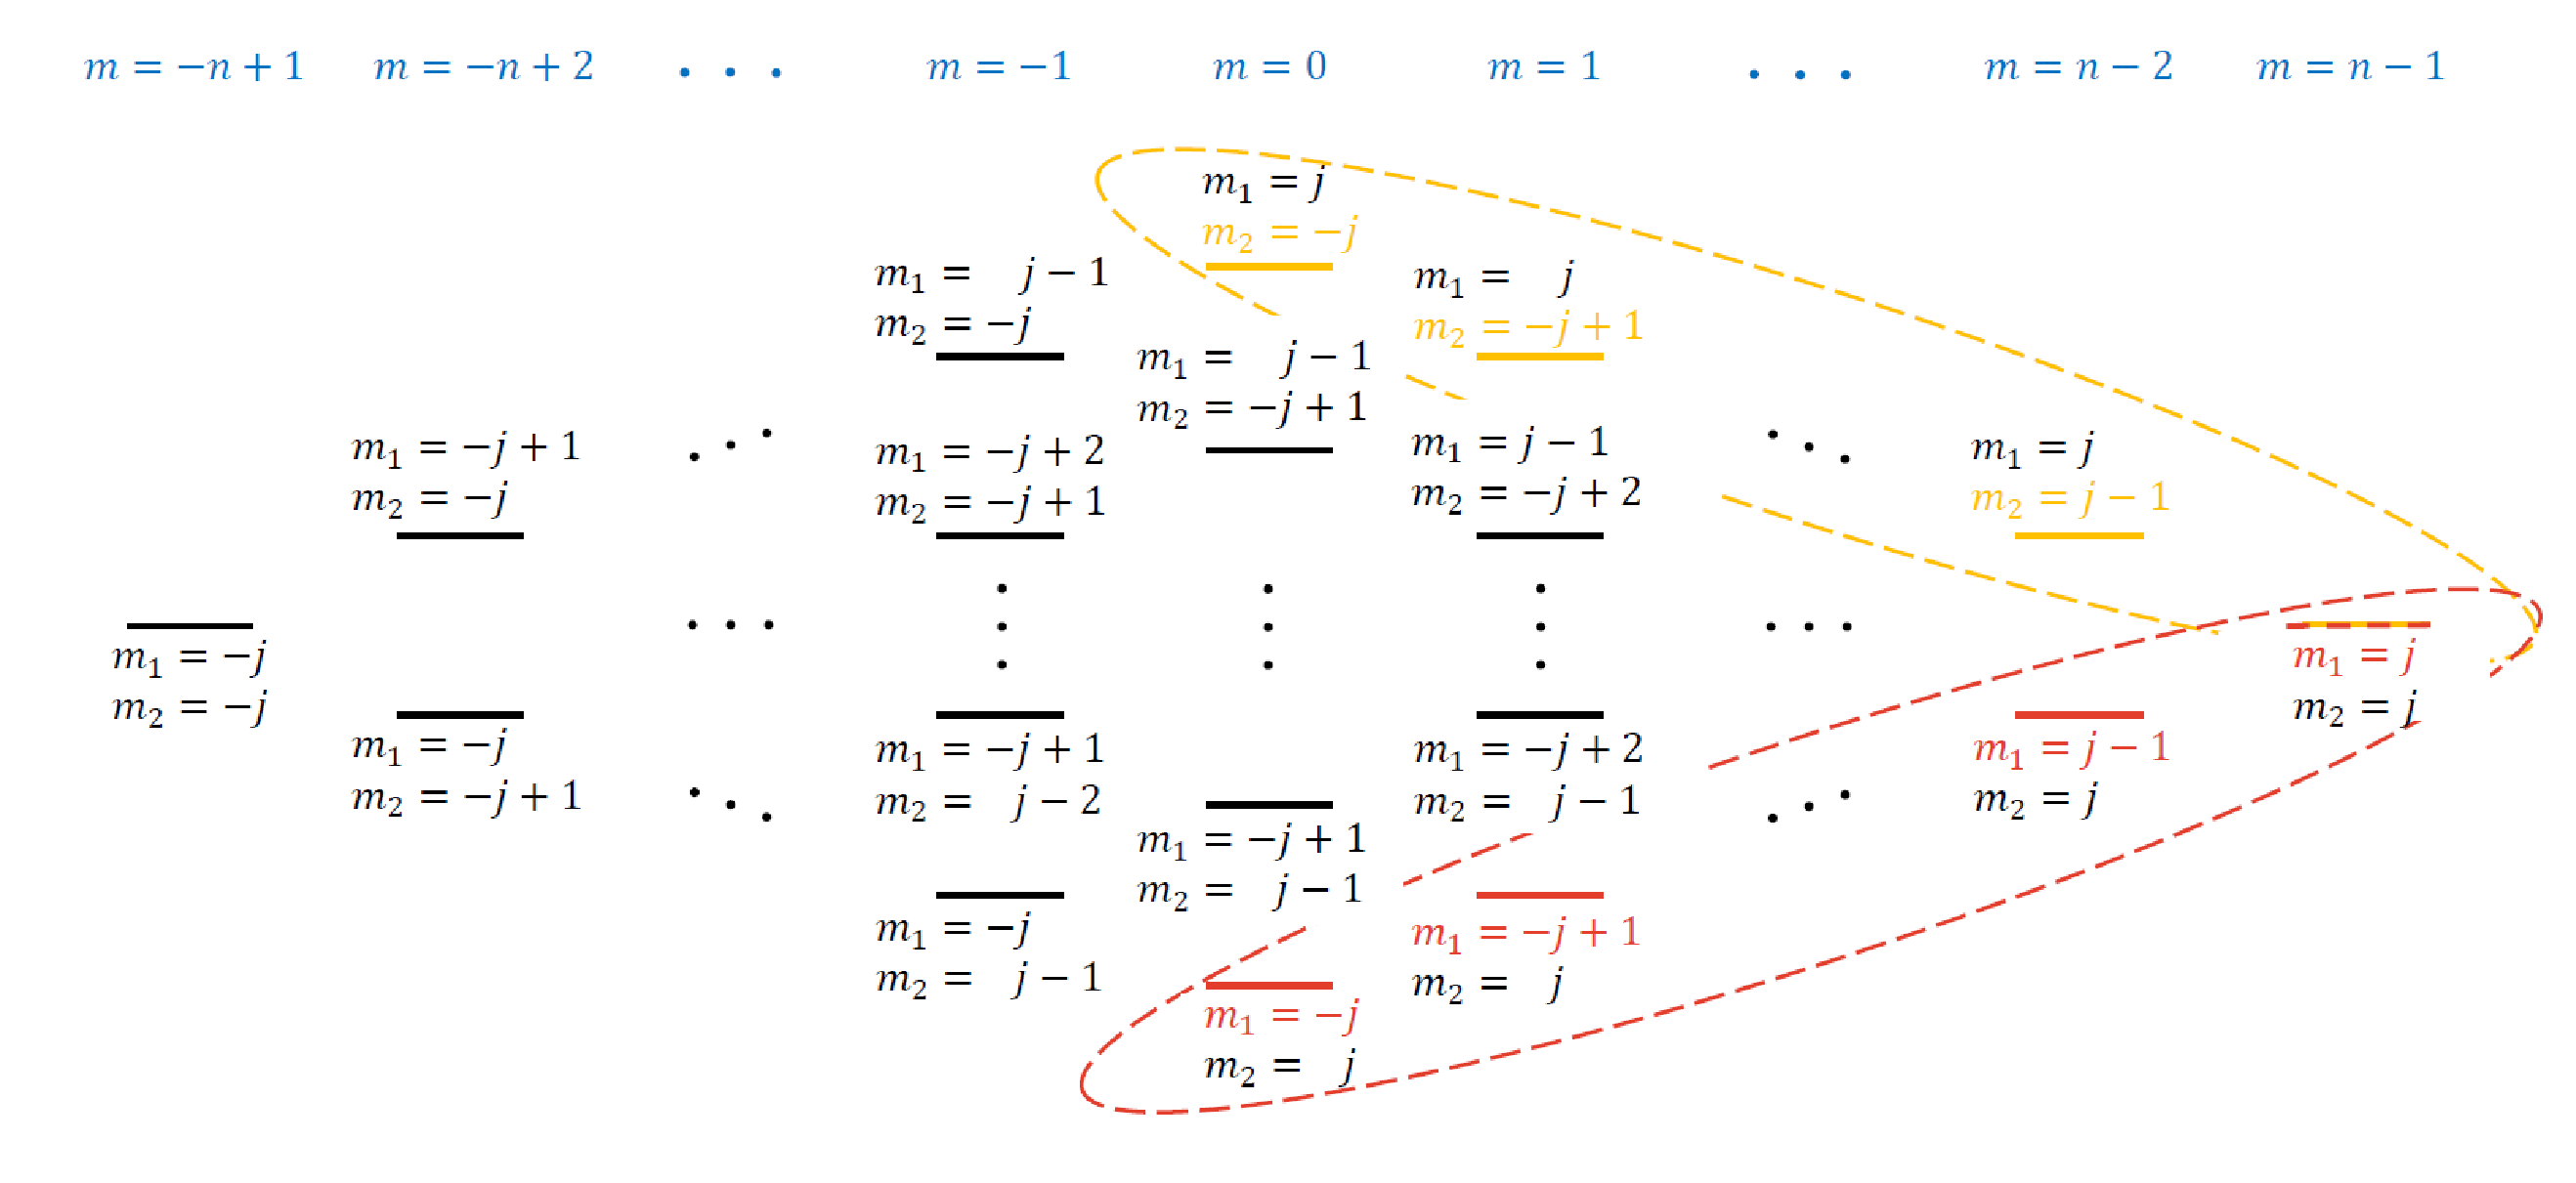
\includegraphics[width=1.\linewidth]{figures/echelle_parabolique_m1m2}
\caption[Échelle des niveaux paraboliques $\ket{n,m_1,m_2}$]{
Niveaux paraboliques $\ket{n,m_1,m_2}$ de même nombre quantique principal $n$, classés horizontalement en fonction de leur nombre quantique magnétique $m=m_1+m_2$. Le nombre $j=j_1=j_2$ est la valeur des moments cinétiques $\hat{\vec{J}}_1$ et $\hat{\vec{J}}_2$ et vaut $j=(n-1)/2$.
La diagonale jaune représente la direction de variation de $m_2$ à $m_1$ fixé et la diagonale rouge la direction de variation de $m_1$ à $m_2$ fixé.
}
\label{fig:parab_m1m2}
\end{figure}


%L'équation de Schrödinger peut s'écrire dans les coordonnées paraboliques $(\xi ,\eta ,\phi )$ obtenues à partir des coordonnées sphériques $(r,\theta ,\phi)$ par la transformation :
%\begin{equation}\label{eq:coordParab}
%\hfill \xi = r(1+\cos\theta) \hfill \eta = r(1-\cos\theta)\hfill
%\end{equation}
%Dans ce système de coordonnées, l'équation de Schrödinger est séparable à condition d'introduire les nombres quantiques $n_1$ et $n2$.
%La base des états paraboliques s'obtient en introduisant les nombres quantiques paraboliques $n_1$ et $n_2$ qui sont fonction de $m_1$ et $m_2$.
%Nous préférerons ici une autre approche pour la plus grande simplicité avec laquelle elle permet de représenter les états atomiques.
%Introduisons à cet effet

Afin d'aider à la représentation des états atomiques, introduisons un nouveau nombre quantique $k=m_1-m_2$, qui quantifie l'excentricité de l'orbite électronique et permet de transformer la base $\ket{n,m_1,m_2}$ en la base $\ket{n,m,k}$ :
\begin{equation}\label{eq:base_nmk}
\left\{
\begin{aligned}
&n \text{ \begin{small}
le nombre quantique principal
\end{small}}\\
&m \text{ \begin{small}
le nombre quantique magnétique variant de
\end{small} }
(-n+1)~~ \text{ \begin{small} à \end{small}} ~~(n-1)\\
&k=m_1-m_2 \text{ \begin{small} variant de\end{small} } (-m-n+1)~~ \text{ \begin{small} à \end{small} } ~~(-m+n-1).
\end{aligned} \right.
\end{equation}
%


\begin{figure}[!h]
\centering
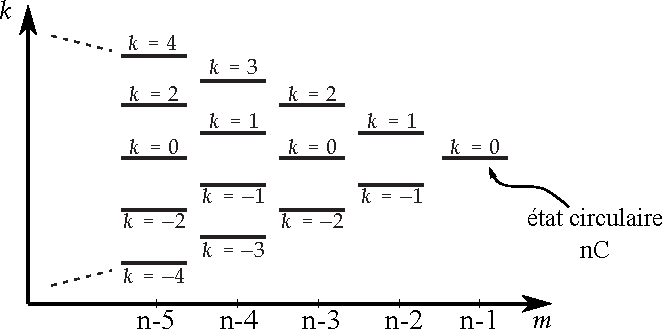
\includegraphics[width=.7\linewidth]{figures/echelle_parabolique_mk}
\caption[Échelle des niveaux paraboliques $\ket{n,m_1,m_2}$]{
Niveaux paraboliques $\ket{n,m,k}$ de même nombre quantique principal $n$, classés horizontalement en fonction de leur nombre quantique magnétique $m$ et étiqueté selon le nombre quantique $k$.
Seuls les niveaux de très grand $m$ sont représentés.
}
\label{fig:parab_mk}
\end{figure}

\noindent La figure \eqref{fig:parab_mk} propose une représentation schématique des niveaux $\ket{m,k}$ de $m$ très élevé au sein d'une multiplicité $n$.

Le niveau de $m$ maximal dans une multiplicité donnée, $\ket{n,m=n-1,k=0} =\ket{n,l=n-1,m=l}$, est appelé le niveau circulaire nC.
Sa fonction d'onde électronique se réduit à un tore éloigné du c\oe ur atomique, de rayon $\sim n(n-1)a_0$, et contenu dans le plan perpendiculaire à l'axe de quantification.
La figure \eqref{fig:wavefunc50C} montre la probabilité de présence $r^2|R(r)|^2$ de l'électron dans le plan perpendiculaire à l'axe de quantification, pour le niveau de Rydberg nC. Celle-ci a une valeur moyenne valant $\sim n^2 a_0$.
Les niveaux de $m$ élevé mais non maximal seront appelés niveaux elliptiques en raison de la forme de leurs fonctions d'onde et seront étiquetés sur la base $\ket{n,m,k}$.
\begin{figure}[!h]
	\centering
	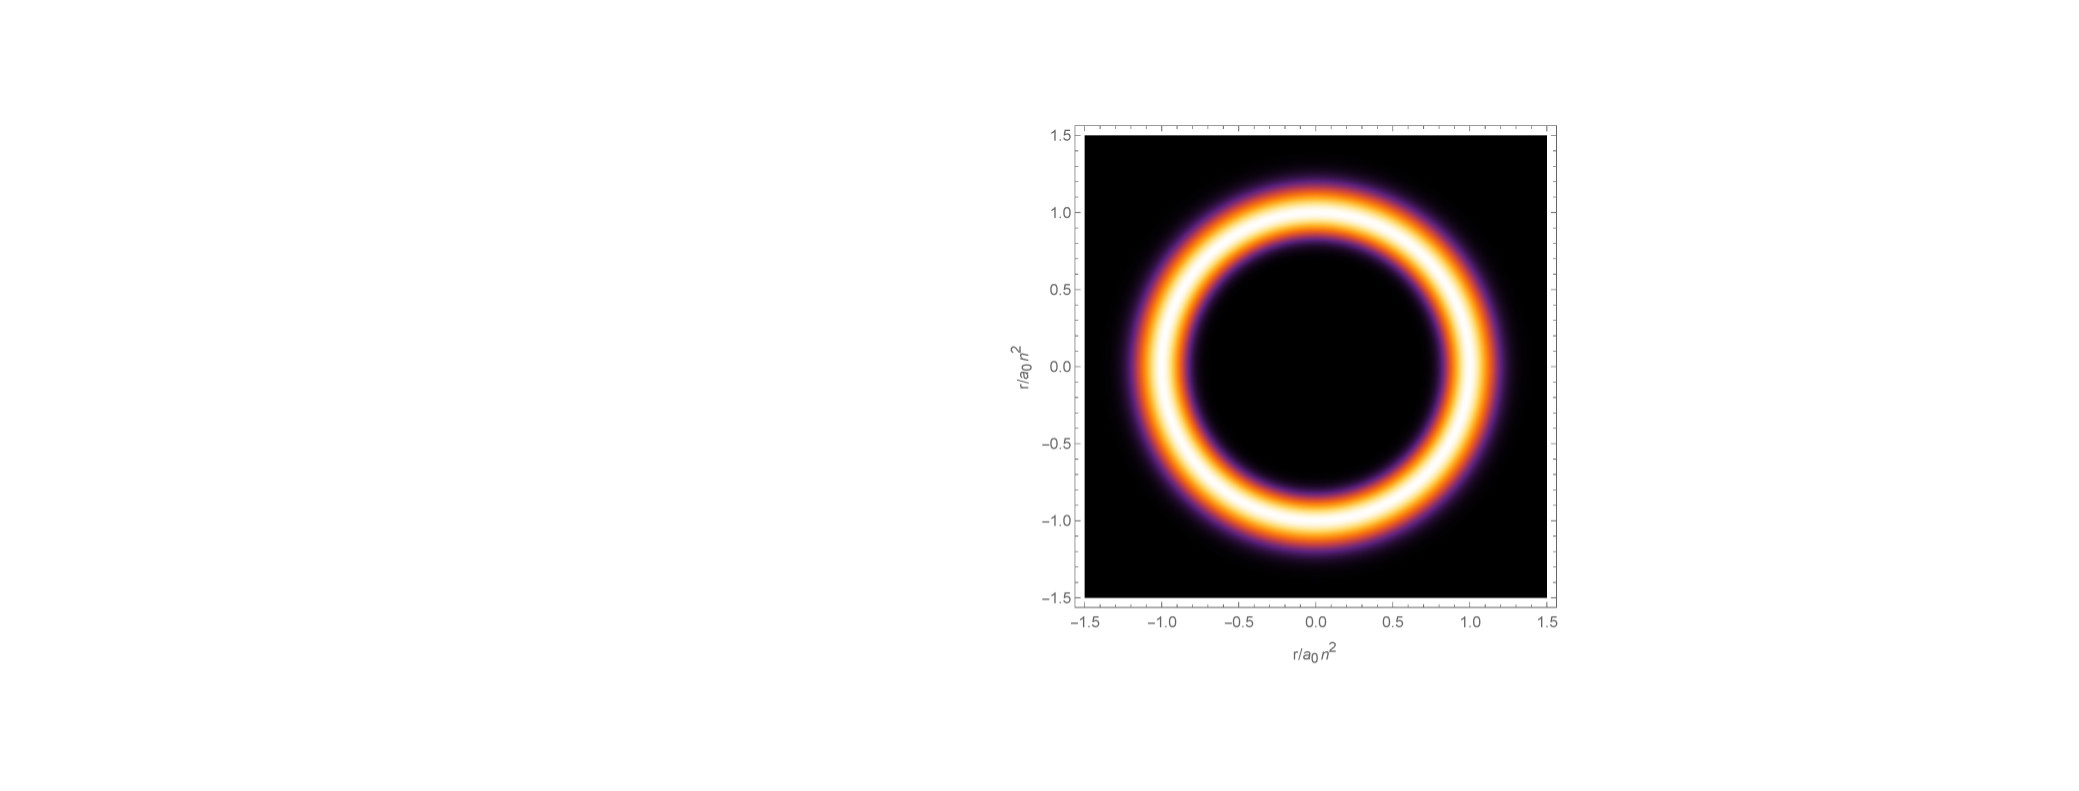
\includegraphics[width=0.6\linewidth]{figures/WaveFunc_50C_}
	\caption[Fonction d'onde du niveau nC]{Probabilité de présence de l'électron dans le niveau nC : $r^2\times |R_{n\mathrm{C}}(r)|^2$.
	Celle-ci décrit un tore de rayon $n^2a_0$ autour du c\oe ur atomique.}
	\label{fig:wavefunc50C}
\end{figure}


\subsection{Le niveau de Rydberg 50C : $\mathbf{\ket{n=50,l=49,m_l=49}}$}
%	Le cas des niveaux circulaires est assez différent. En effet, ceux-ci sont définis par leur moment cinétique orbital maximal $l=n-1$, ainsi que par la projection de ce moment cinétique sur l'axe de quantification, elle aussi maximale : $|m_l| = l = (n-1)$.
%	Cela amène à une orbitale électronique qui se réduit à un tore, éloigné du c\oe ur atomique et contenu dans le plan perpendiculaire à l'axe de quantification du moment cinétique. La figure \eqref{fig:wavefunc50C} montre la probabilité de présence de l'électron dans le niveau de Rydberg 50C.	
%\begin{figure}[!h]
%	\centering
%	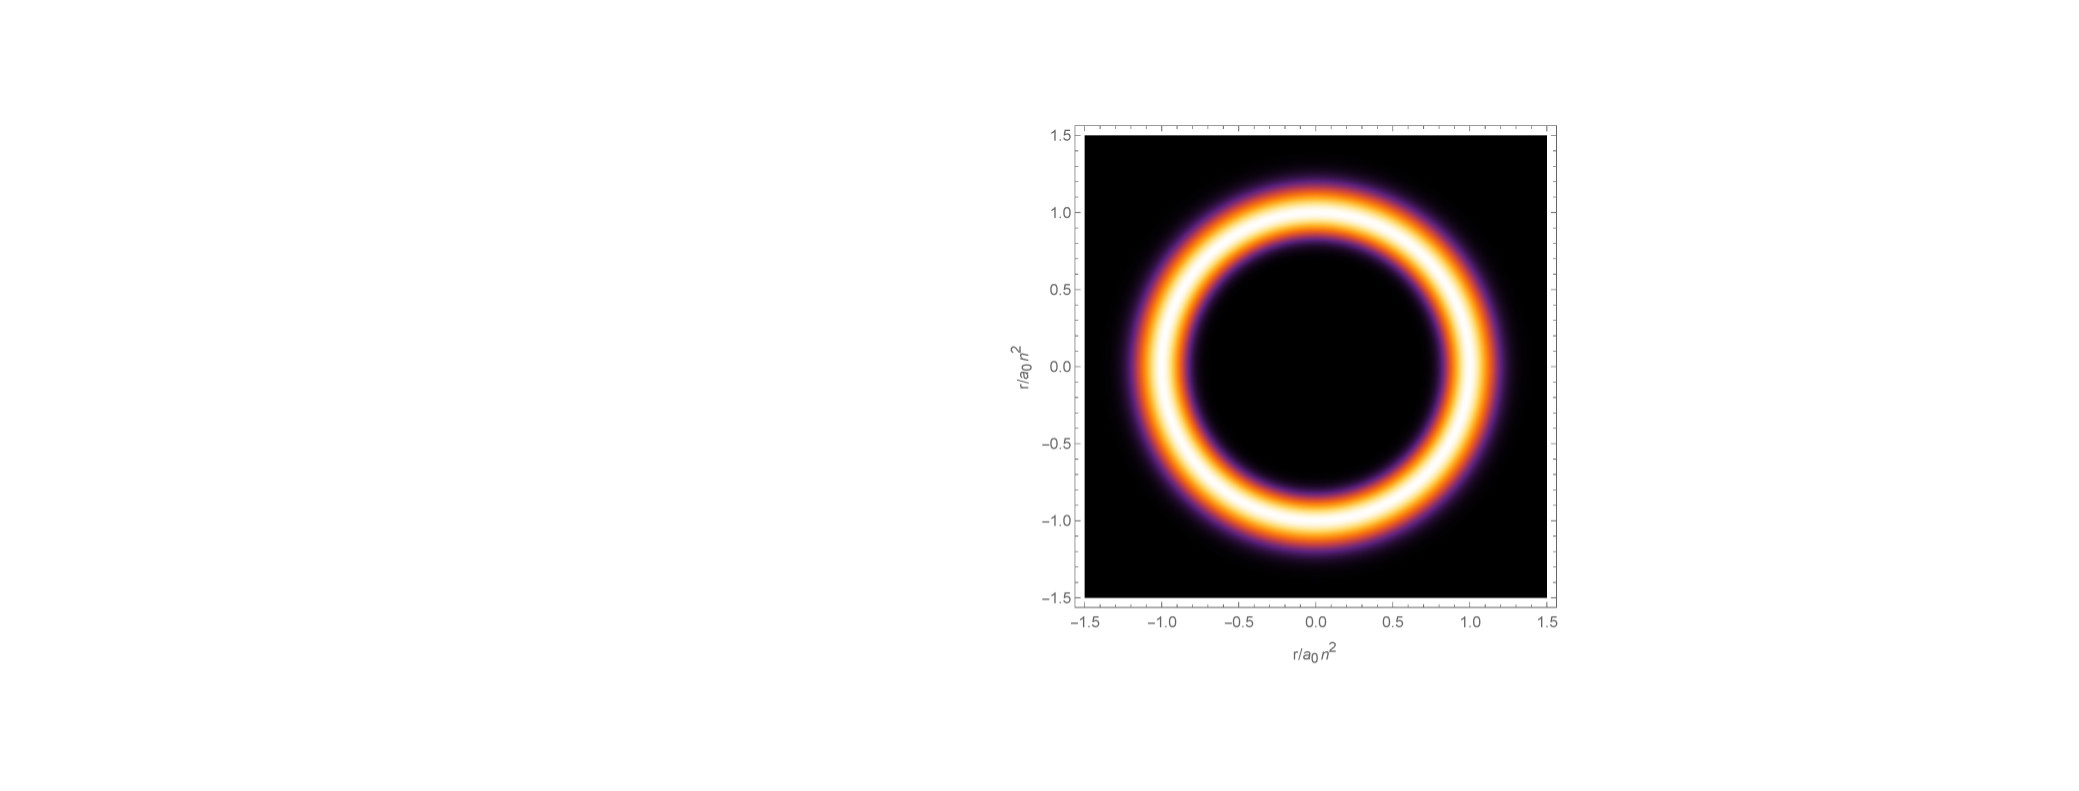
\includegraphics[width=0.6\linewidth]{figures/WaveFunc_50C_}
%	\caption[Fonction d'onde du niveau 50C]{Probabilité de présence de l'électron dans le niveau 50C : $r^2\times |R_{50\mathrm{C}}(r)|^2$.}
%	\label{fig:wavefunc50C}
%\end{figure}
%La méthode de Numerov permet de calculer le rayon moyen de cette orbitale électronique,
%\begin{equation}
%\braket{r}_{50\mathrm{C}} = 2500~a_0 = \numv{132}\si{\nano\meter},
%\end{equation}
%mais il est intéressant de noter que la partie radiale de la fonction d'onde se réduit à une expression analytique simple pour les niveaux circulaires.
%
%La dérivation de cette expression mène rapidement à l'affirmation que le maximum de $r^2|R_{nC}(r)|^2$ se situe exactement en $n^2 a_0$ et, étant donnée la forme de $r^2|R_{nC}(r)|^2$, que
%\begin{equation}\label{eq:rayon_nC}
%\braket{r}_{n\mathrm{C}} \simeq n^2\times a_0.
%\end{equation}

Parmi les niveaux de Rydberg circulaires, le niveau 50C sera d'un intérêt particulier pour nous.
Dans le cas du niveau 50C, cela donne $\braket{r}_{50C} \simeq 50^2 a_0 = 2500 a_0 = \numv{132}\si{\nano\meter}$.
	
%Ici, la transition entre le niveau $50C$ et le niveau $49C=\ket{n=49,l=48,m_l=48}$ vaut $E/h = \numv{54.25955}\si{\giga\hertz}$.

En ce qui concerne leut temps de vie, les niveaux de Rydberg circulaires ont une différence essentielle avec les niveaux de faible $l$ : les niveaux circulaires n'ont de transition dipolaire possible que vers des niveaux eux aussi à très grand $l$, et donc à très grand $n$.
Il n'y a d'ailleurs qu'une seule transition spontanée possible depuis le niveau $\ket{n,l=n-1,m_l=l}$, c'est celle vers le niveau circulaire $\ket{n'=n-1,l'=n'-1,m_l'=l'}$.
En effet, il n'existe aucun niveau de plus basse énergie que $nC$ mais qui aurait un $l$ qui lui soit égal ou supérieur.
La figure \eqref{fig:spontem_50C49C} représente les schémas de niveaux près de l'état circulaire $n=50$ et met en évidence l'absence de toute autre transition par émission spontanée depuis le niveau 50C.
Le niveau 50C ne peut donc se désexciter spontanément que vers le niveau 49C, ce qui réduit considérablement la contribution de l'émission spontanée à son taux de désexcitation radiative.
Le calcul du dipôle de transition $\braket{50\text{C}|\hat{\vec{d}}|49\text{C}}$ par la méthode de Numerov donne une valeur de $\numv{1704.71} e a_0$.
En appliquant l'équation \eqref{eq:EinsteinAif} à la fréquence de transition de $\SIv{54.25955}{\giga\hertz}$, on obtient un taux de désexcitation valant $\Gamma_{50C}(\SIvv{0}{\kelvin}) = A_{50C-49C} = \SIv{34.9056}{\hertz}$.
Le temps de vie à température nulle du niveau 50C est donc de $\tau_{0,50C} = \SIv{28.65}{\ms}$, soit cent fois plus que celle du niveau 60S.
\begin{figure}
	\centering
	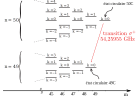
\includegraphics[width=0.7\linewidth]{figures/spontem_50C49C}
	\caption[Schéma de niveaux 50C-49C]{Schéma de niveaux des multiplicités $n=50$ et $n=49$ près des niveaux 50C et 49C. La seule transition possible par émission spontanée depuis le 50C est la transition vers le 49C.}
	\label{fig:spontem_50C49C}
\end{figure}

%La limitation de la durée de vie du niveau 50C provient donc en premier lieu de l'absorption et de l'émission stimulée par le rayonnement du corps noir vers les niveaux accessibles par transition dipolaire électrique.
Étant donné le faible taux de désexcitation spontanée du niveau 50C, l'effet du rayonnement du corps noir sur sa durée de vie sera important dès les très basses températures.
Le rayonnement du corps noir amplifiera non seulement le taux de désexcitation vers le niveau 49C, mais autorisera également par absorption les transitions vers les niveaux de $n$ supérieur.
Ainsi, alors que la réduction du temps de vie du niveau 60S entre $\numv{0}\si{\kelvin}$ et $\numv{4.2}\si{\kelvin}$ est faible (voir table \ref{tab:lifetime_60S}), la réduction du temps de vie du niveau 50C entre $\numv{0}\si{\kelvin}$ et $\numv{4}\si{\kelvin}$ sera bien plus importante.
\`A température ambiante de $\numv{300}\si{\kelvin}$, la durée de vie de 50C tombe en effet à $\numv{122}\si{\micro\second}$, très similaire à celle du niveau 60S.
La figure \eqref{fig:lifetime_50C} montre l'évolution de la durée de vie du niveau 50C en fonction de la température de rayonnement du corps noir, calculée à partir des équations \eqref{eq:EinsteinBif} et \eqref{eq:BoseStat}.

\begin{figure}[!h]
	\centering
	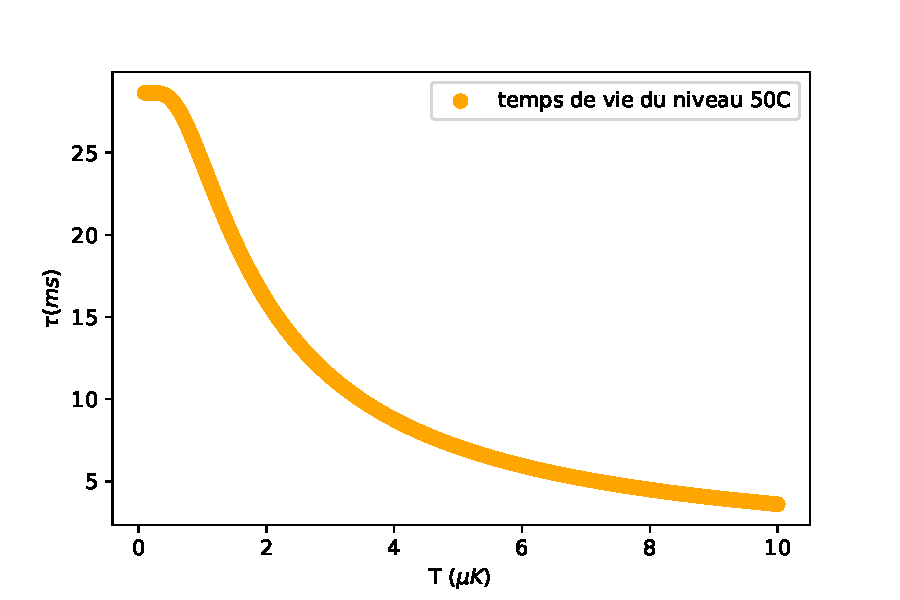
\includegraphics[width=0.6\linewidth]{figures/lifetime_50C}
	\caption[Durée de vie du niveau 50C]{Durée de vie radiative du niveau de Rydberg 50C en fonction de la température de rayonnement du corps noir.}
	\label{fig:lifetime_50C}
\end{figure}


\bigskip

Nous avons désormais une bonne connaissance des caractéristiques des atomes de Rydberg individuels, en particulier dans les niveaux 60S et 50C.
Ce sont de très grands atomes, avec de très grands moments dipolaires de transition, et un temps de vie très long.
Comment se comportent ces atomes de Rydberg lorsqu'ils ne sont plus isolés mais proches les uns des autres ?

%\section{Atomes de Rydberg en interaction}
%	\subsection{Deux atomes de Rydberg}
%		\noindent hamiltonien d'interaction entre deux dipôles
%		\[
%		V_{dd} = \frac{1}{4\pi\epsilon_0 r^3} \left( \mathbf{d_1}\cdot \mathbf{d_2} - 3(\mathbf{d_1}\cdot \frac{\mathbf{r}}{r})(\mathbf{d_2}\cdot\frac{\mathbf{r}}{r}) \right)
%		\]
%		\noindent de l'interaction dipole-dipole générale au terme de Van der Waals en $1/r^6$ \\
%		\noindent terme d'énergie et terme d'échange
%	\subsection{les interactions entre Rydberg de bas $l$}
%		\noindent origine du $C_6$ pour 60s-60s et $C_6/A_6$ avec les voisins\\
%		reprendre Raul.figI.3 qui présente la partie radiale du dipôle 60s-ns en fonction de n\\
%		\noindent principe du blocage dipolaire et facilitation (rapide)
%	\subsection{les interactions entre Rydberg circulaires}
%		\noindent $C_6$ pour 50c-50c et $C_6/A_6$ avec les voisins \\
%		\noindent attention à l'anisotropie\\
%		équivalent de la figure ci dessus (Raul.figI.3) pour les 50c, à modifier pour l'anisotropie
